\chapter{Конструкторский раздел}
В этом разделе будут приведены схемы реализации алгоритмов, 
а также способы тестирования и выделения классов эквивалентности.

\section{Схемы алгоритмов}
На рисунке 2.1 будет приведена схема реализации алгоритма сортировки пузырьком.
На рисунке 2.2 будет приведена схема реализации алгоритма сортировки вставками.
На рисунке 2.3 будет приведена схема реализации алгоритма сортировки выбором.

\begin{figure}[hp]
	\begin{center}
		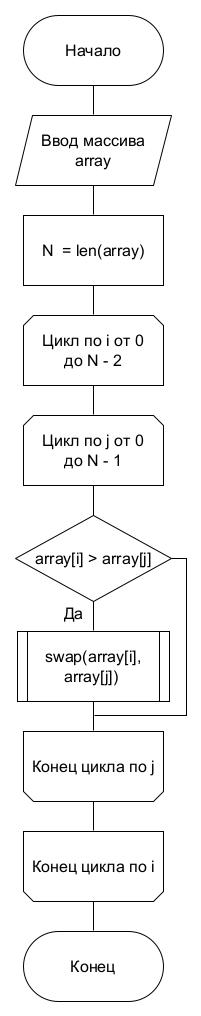
\includegraphics[height=23cm]{graph/bubble.jpg}
	\end{center}
	\caption{Схема алгоритма сортировки пузырьком}
\end{figure}

\begin{figure}[hp]
	\begin{center}
		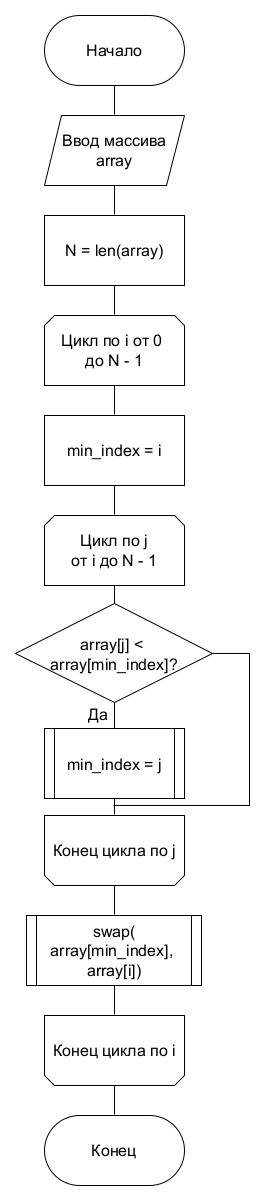
\includegraphics[height=23cm]{graph/select.jpg}
	\end{center}
	\caption{Схема алгоритма сортировки выбором}
\end{figure}

\begin{figure}[hp]
	\begin{center}
		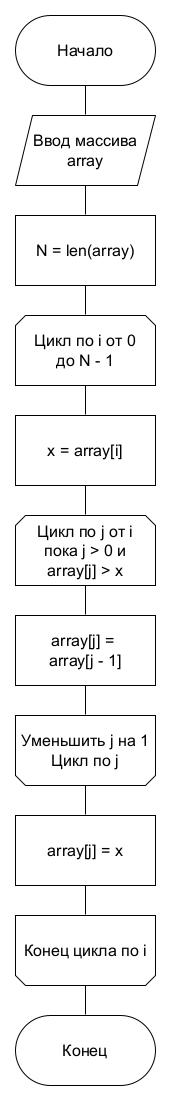
\includegraphics[height=23cm]{graph/insert.jpg}
	\end{center}
	\caption{Схема алгоритма сортировки вставками}
\end{figure}

\clearpage

\section{Типы данных для алгоритмов}
Тестирование алгоритмов будет производиться на целых числах, 
которые могут быть и отрицательными, и равны нулю. Несмотря на это,
сами реализации алгоритмов универсальны и предназначены для любых численных типов данных.

Размер массива может быть произвольным.

\section{Способ тестирования}
Тестирование программы будет произодиться методом чёрного ящика.
Такой подход выбран, так как от реализаций алгоритмов требуется в первую
очередь правильность работы.
Сама по себе реализация не требует тестировки, так как в точности
повторяет теоретические принципы, сформированные в аналитическом
разделе.

В качестве классов эквивалентности были выбраны следующие сущности:
\begin{itemize}
	\item массив из случайных элементов;
	\item отсортированный по возрастанию массив;
	\item отсортированный по убыванию массив;
	\item массив, состоящий из одинаковых элементов;
	\item массив нулевой длины;
	\item массив единичной длины;
	\item массив, в котором несколько одинаковых элементов;s
\end{itemize}

Для корректного сравнения требуется для каждой реализации сортировки
сравнить полученный на выходе массив с эталонным результатом массива.

\section{Вывод}
Были приведены схемы алгоритмов, рассмотрены типы данных
для алгоритмов, а также описан способ тестирования.